%% LyX 1.6.7 created this file.  For more info, see http://www.lyx.org/.
%% Do not edit unless you really know what you are doing.
\documentclass[english]{article}
\usepackage[T1]{fontenc}
\usepackage[latin9]{inputenc}
\usepackage{float}
\usepackage{amsmath}
\usepackage{graphicx}
\usepackage{amssymb}

\makeatletter

%%%%%%%%%%%%%%%%%%%%%%%%%%%%%% LyX specific LaTeX commands.
%% A simple dot to overcome graphicx limitations
\newcommand{\lyxdot}{.}


\makeatother

\usepackage{babel}

\begin{document}

\title{YCP Robot}


\author{Tori Bare, Cory Boyle, Jason Cluck, Drew Wicke}


\date{November 21 2011}
\maketitle
\begin{abstract}
The objective of the project was to build software to make X80SVP
robot autonomous. To produce autonomy, the software controls the robot
by avoiding obstacles and producing a wandering type behavior. Software
was also writen to utilize Microsoft's Kinect to provide gesture recognition
to operate the robot. Finally, in order to provide a suitable test
environment a 3D virtual simulator was created that can simulate a
robot with sensor and motor funcionallity. Using the Robot Operating
System (ROS), algorithms were developed for obstacle avoidance, and
3D navigation. Additionally, a simulator was created in OpenGL that
was used as a testbed for these algorithms.
\end{abstract}

\part*{Introduction}

The objective of the project was to build software to make a robot
autonomous. To produce autonomy the software controls the robot by
avoiding obstacles and producing a wandering type behavior. The next
goal achieved was to control the robot using gesture recognition.
Finally, in order to provide a suitable test environment a 3D virtual
simulator was created that can simulate a robot and its sensor and
motor funcionallity.

One of the goals of the Robot Operating System (ROS) is to provide
roboticists a software platform for specific robots. ROS is beneficial
in this way because it creates \textquotedblleft{}a wide variety of
frameworks to manage complexity and facilitate rapid prototyping of
software for experiments, resulting in the many robotic software systems
currently used in academia and industry\textquotedblright{}\cite{quigley:ROSopensourceRobotOperatingSystem}.
This paper addresses the construction of a new ROS package that controls
the X80SVP robot. The package, which already implements obstacle avoidance
and wandering behavior, provides low level drivers up to a robust
development framework that can be extended.



Another goal of the ROS community is to provide simulation software
to test the robot. For example, the player project consists of Player,
a robot interface, Stage, a two-dimensional robot simulator, and Gazebo,
a three-dimensional robot simulator. As part of the project a new
simulator for ROS was developed that can be extended and provides
a Kinect sensor.

The first part provides a background detailing the devices, algorithms
and libraries that were used; the second part discusses the design
of the system following with implementation details; finally, it concludes
with an overview of future work.


\part*{Background}

Various devices, technologies and algorithms were used to create an
autonomous robot. The robot that was used was an X80SVP. It was chosen
because this was the robot that was being considered for use in a
future robotics course at YCP. A Beagleboard hosted the software and
acted as a bridge to the robot while the Robot Operating System provided
a framework for the software. Braitenburg aggression behavior was
used to provide obstacle avoidance and a Kinect was used to provide
vision. Lastly, OpenGL was used to provide 3D graphics for the simulator.


\section*{Devices}

The X80SVP Robot has a max speed of 75 cm/s, weighs 3.5 kg, has a
max payload of 15 kg, and has a three hour battery life. The robot
also has IR and ultrasonic range sensors, as well as pyro-electric
human motion sensors as seen in Figure \ref{fig:X80SVP-Robot}.

%
\begin{figure}[H]
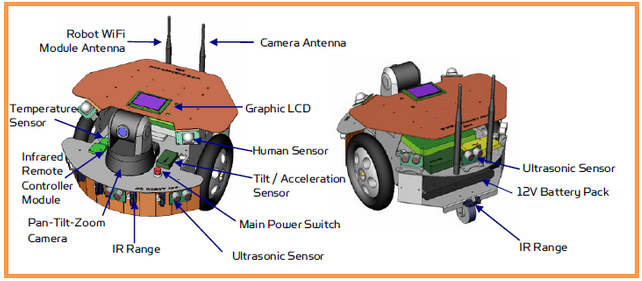
\includegraphics[scale=0.75]{images/X80SVPRobot}

\caption{\label{fig:X80SVP-Robot}X80SVP Robot \cite{:XSVPQuickStartGuide}}



\end{figure}


The Beagleboard XM was chosen as the computer for the X80SVP. The
Beagleboard has many peripheral options, a 1 GHz CPU, a DSP, and it
is very popular in the open source/ROS communities. The initial plan
accounted for the DSP being able to process the Kinect vision data
while the CPU handled the overhead associated with ROS. The major
components on the board are shown below in Figure \ref{fig:Beagleboard's-Main-Components}.

%
\begin{figure}[H]
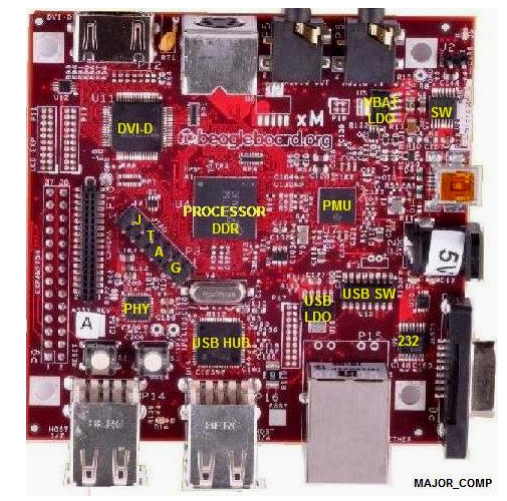
\includegraphics[scale=0.4]{images/beagleboardMajorComps}

\caption{\label{fig:Beagleboard's-Main-Components}Beagleboard's Main Components
\cite{:BeaglSysteReferManua}}

\end{figure}


A Kinect was used to generate maps of the robot's surroundings and
to allow the robot to navigate intelligently through his environment.
The OpenNI drivers for ROS, created by the makers of the Kinect, would
enable the Kinect to be used in this manner. One of the main concerns
with using the Kinect was the processing power that it would require.
The Kinect produces a message that is roughly 1 MB at a rate of 30
frames per second, this equates to the Kinect sending about 30 MB
of data each second. At first, it was expected that the DSP on the
Beagleboard would have been able to handle the Kinect\textquoteright{}s
processing; however, due to the overhead of ROS, the processing will
most likely have to be offloaded to a netbook. 


\section*{ROS}

ROS is a framework that facilitates the construction and execution
of applications for robots. {}``It provides hardware abstraction,
device drivers, libraries, visualizers, message-passing, package management,
and more'' \cite{ros}. There are implementations of ROS in C++,
Python, Lisp, Octave, and Java. ROS was chosen to act as the framework
for the project because it provides a good communication model, a
well structured programming environment, and an implementation in
Java.

ROS executables are called nodes and are the main source of communication.
ROS provides a master node called Ros Master that oversees running
nodes and a parameter server, it also acts as the matchmaker for nodes
and topics as seen in figure \ref{fig:RosMaster}. ROS nodes can communicate
using topics, which are similar to named busses which offer a publisher/subscriber
type communication model. Nodes publish messages on topics which other
nodes can subscribe to in order to receive the information being published.
However, the nodes only know the name of the topic and not the name
of the other node as seen in figure \ref{fig:RosMaster}. A message's
fields are described using the YAML language, a {}``human friendly
data serialization standard for all programming languages'' \cite{::YYAML}.
ROS can then convert the message file into a file that the targeted
language can use, such as a header file in C++. ROS uses this message
passing communication model because it is language independent and
allows for {}``unidirectional, streaming communication''\cite{ros}.

%
\begin{figure}[H]
\begin{centering}
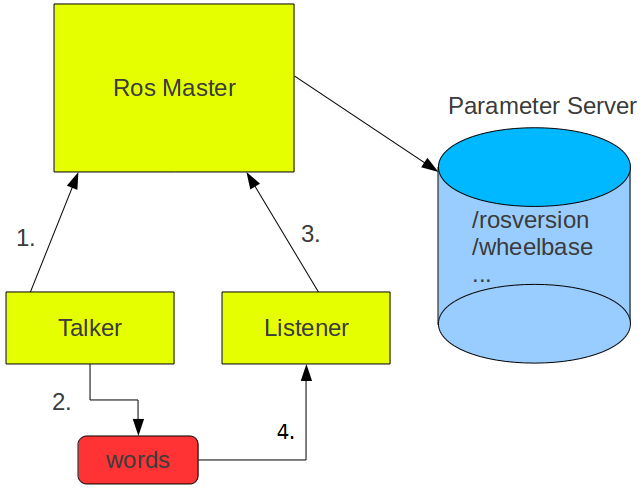
\includegraphics[scale=0.35]{images/RosMaster}
\par\end{centering}

\caption{\label{fig:RosMaster}1. The Talker node tells ROS Master that it
wants to publish to the words topic. 2. Then Talker starts publishing
to the words topic. 3. Listener tells Ros Master that it wants to
subscribe to the words topic. 4. Ros Master pairs Talker and Listener
so that Listener can start receiving messages on the words topic.
The Parameter Server is similar to a registry in that it stores state
information which nodes can access.}

\end{figure}


ROS also provides a hierarchical packaging based structure to group
common elements as seen in figure \ref{fig:RosStackHierarchy}. Nodes,
the executables, that have similar roles are grouped into a package.
Packages that share a common purpose are grouped into a stack. Stacks
can contain one or more packages. Therefore, ROS's goal is to build
a complex system out of simple, single-purpose parts\cite{ros}.

%
\begin{figure}[H]
\begin{centering}
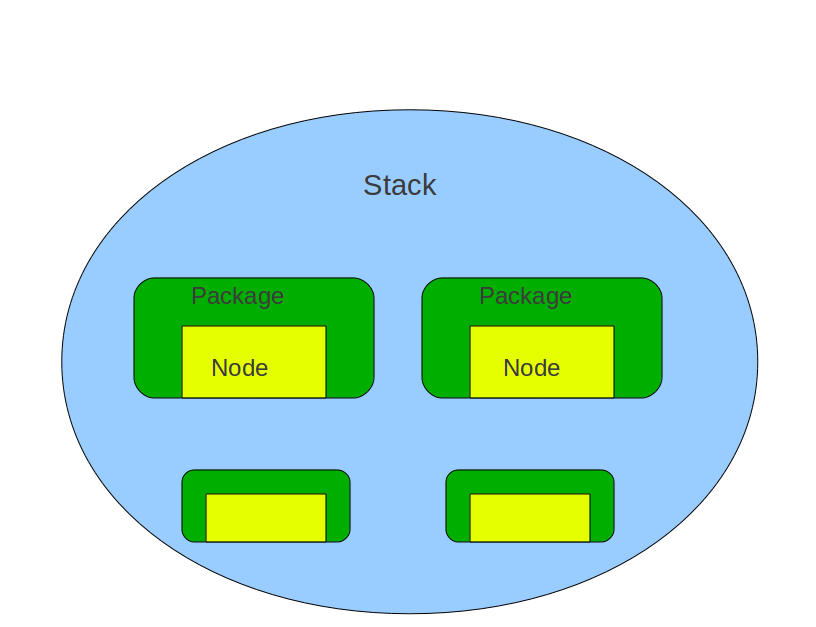
\includegraphics[scale=0.25]{images/ColorRos}
\par\end{centering}

\caption{\label{fig:RosStackHierarchy}An illustration of the hierarchical
structure of ROS. There are no limits on the number of packages per
stack and no limit on the number of nodes per package.}



\end{figure}


Java's object oriented structure complements ROS's goal of complexity
out of simplicity. The rosjava stack is the first implementation of
ROS in Java and {}``developed at Google in cooperation with Willow
Garage'' \cite{rosjava}. It was chosen to allow future students
in robotics the ease of use that Java provides, as well as for Java's
cross platform capability. The rosjava implementation is similar to
the other ROS implementations in that it provides the same communication
framework and packaging structure. However, in order to integrate
with other languages ROS messages are converted to classes and stored
into Java jar files. The jar files can then be imported a class and
the messages data types can then be used in communication over topics.
Unlike other implementations, rosjava also provides its own ROS master
allowing it to run on devices that only allow Java, such as an Android
phone.


\section*{Obstacle Avoidance Algorithm}

There are two main ways to implement obstacle avoidance, motor fusion
and sensor fusion. Motor fusion also termed reactive control uses
a direct correlation from sensor readings to motor velocities without
any intermediate representation, such as a map\cite{driankov2001fuzzy}.
The main advantage to using motor fusion is its ability to function
well in real time systems. Motor fusion or {}``reactivity is essential
for any system operating in a dynamic, uncertain environment''\cite{rosenblatt2007centralized}.
However, when a robot has many sensors which map to a motor command
the processing time increases and therefore decreases the usefulness
of motor fusion. 

Sensor fusion uses the sensor data to reconstruct the surroundings
to produce motor commands. The reconstruction could be in the form
of a map of the environment which can then be used to avoid obstacles
and possibly provide for higher level goals. Therefore, sensor fusion
provides higher level functionallity than motor fusion. However, the
main disadvantage of sensor fusion is due to translating the sensor
data from various sensor sources which {}``further complicates the
selection of methods, uncertainty representations, and assessments
of performance'' \cite{kam1997sensor}.

For the X80SVP robot, obstacle avoidance was accomplished by a motor
fusion algorithm utilizing Braitenburg's aggression behavior. Motor
fusion was chosen because the robot's sensors were unreliable and
limited therefore making the sensor fusion model inappropriate. Also,
Braitenburg's algorithm does not rely on the type or variety of range
sensors to provide obstacle avoidance. 

Braitenburg behaviors are a form of synthetic psychology described
in\cite{braitenberg1986}. These behaviors were thought experiments
into how different emotions, such as fear, aggression, and love, can
provoke movement based on sensor stimulation. Aggression behavior
is caused by pairing the sensors and motors on opposite sides through
a non-decreasing function as seen in figure \ref{fig:Braitenberg-agression-behavior}.

%
\begin{figure}[H]
\begin{centering}
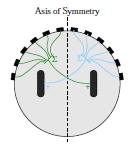
\includegraphics[scale=0.8]{images/AgressionRobot}
\par\end{centering}

\caption{\label{fig:Braitenberg-agression-behavior}Braitenberg aggression
behavior \cite{ran2005obsavothrbraaggbehmotfus}.}

\end{figure}


To implement aggression behavior for obstacle avoidance, only the
front sensors are used and also modifications to use a centered sensor
were made to the algorithm presented in \cite{ran2005obsavothrbraaggbehmotfus}.
The algorithm computes both the linear and angular velocity for the
robot given the normalized sensor readings as shown in equations \ref{eq:translationalSpeed}
and \ref{eq:rotationalSpeed}. For example, when the no obstacles
are present the robot will move forward at max velocity. However,
if there is an obstacle that is closer to one side of the robot then
the motor on that side will spike causing the robot to rotate and
avoid the obstacle. Accounting for the center sensor separately allows
the robot to avoid deadlock while in symmetric corners. The value
of a sensor increases as an obstacle gets farther away and as the
velocity becomes greater in that direction, providing a smooth wandering
movement that effectively avoids obstacles.

\begin{equation}
\alpha_{S}(t_{k})=\sum_{i\in L\cup R}w_{i}^{\alpha_{S}}\hat{r}_{i}^{S}(t_{k})\label{eq:translationalSpeed}\end{equation}


\begin{equation}
\beta_{S}(t_{k})=\sum_{i\in R}w_{i}^{\beta_{S}}\mathfrak{D}(\theta'_{i})\hat{r}_{i}^{S}(t_{k})-\sum_{i\in L}w_{i}^{\beta_{S}}\mathfrak{D}(\theta'_{i})\hat{r}_{i}^{S}(t_{k})\label{eq:rotationalSpeed}\end{equation}


$\alpha_{S}$ and $\beta_{S}$ are the normalized translational and
rotational speeds in the range {[}0,1{]} and {[}-1,1{]} respectively.
$w_{i}^{\alpha_{S}}$ and $w_{i}^{\beta_{S}}$ are constant weights
corresponding to the $i^{th}$sensor defined in equations \ref{eq:translationalWeight}
and \ref{eq:rotationalWeight}. $\hat{r}_{i}^{S}(t_{k})$ is the current
normalized filtered range value of the $i^{th}$ sensor. $\mathfrak{D}(\theta'_{i})=90-|\theta_{i}|$
the angular distance. Where $\theta_{i}$ is angle from the x-axis
to the sensor assuming the x-axis lies on the axle and y-axis divides
the robot in half.

\begin{equation}
\mathit{w}_{i}^{\alpha_{S}}=k_{i}^{\alpha}e^{-\frac{\mathfrak{D}(\theta'_{i})^{2}}{2\sigma_{\alpha}^{2}}}\label{eq:translationalWeight}\end{equation}


\begin{equation}
\mathit{w}_{i}^{\beta_{S}}=k_{i}^{\beta}e^{-\frac{\mathfrak{D}(\theta'_{i})^{2}}{2\sigma_{\beta}^{2}}}\label{eq:rotationalWeight}\end{equation}


$k_{i}^{\alpha}$ and $k_{i}^{\beta}$ are normalizing constants so
that the speeds are normalized. $\sigma_{\alpha}^{2}$ and $\sigma_{\beta}^{2}$
are the variance chosen here to be 1400 and 350 respectively in order
to place a greater weight on small angles and less weight on greater
angles as can be seen in figures \ref{fig:LinearWeight} and \ref{fig:AngularWeight}.

%
\begin{figure}[H]
%
\begin{minipage}[t]{0.45\columnwidth}%
\begin{center}
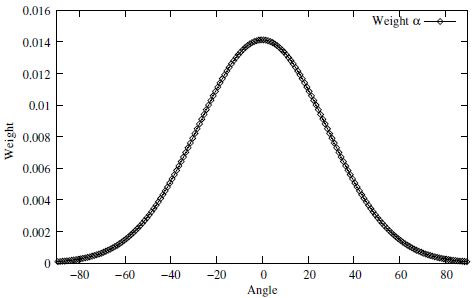
\includegraphics[scale=0.4]{images/linearWeight}
\par\end{center}

\caption{\label{fig:LinearWeight} Weights for $\alpha_{S}(t_{k})$ \cite{ran2005obsavothrbraaggbehmotfus}.}
%
\end{minipage}\hfill{}%
\begin{minipage}[t]{0.45\columnwidth}%
\begin{center}
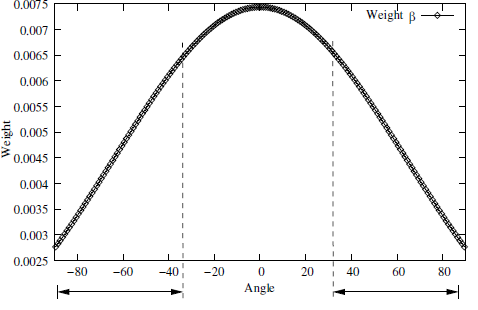
\includegraphics[scale=0.4]{images/angularWeight}
\par\end{center}

\caption{\label{fig:AngularWeight}Weights for $\beta_{S}(t_{k})$ \cite{ran2005obsavothrbraaggbehmotfus}.}
%
\end{minipage}
\end{figure}



\section*{Simulator}

A simulator was developed to fulfill the use case of being able to
test the navigation algorithms in a clean virtual environment before
deploying them to the actual robot. The simulator uses OpenGL to model
the robot and environment. OpenGL generates a depth-map as part of
its rendering process and this is used to compute distances from the
robot in any direction to other objects in the environment. This makes
it possible to simulate virtual versions of the real sensors by rendering
the viewport from the perspective of the sensors and reading the depth-map
to determine the simulated sensor value.

The simulator uses a number of libraries to make the OpenGL API more
manageable. The Free OpenGL Utility Toolkit (freeglut) is used to
provide the basic windowing functions for the GL application. The
OpenGL Utility Library (GLU) provides utility functions for computing
projection matrices, used to create the perspective camera views.
The Simple OpenGL Image Library (SOIL) is used to provide texture-loading
capabilities. The simulator also interfaces directly with the X.Org
Server APIs for some functions in handling mouse and full-screen controls.
A custom loader was written to load DirectX format mesh files as exported
by Blender. This allows environments as well as movable obstacles
of completely arbitrary design and complexity to be modeled quickly,
thus it can be adapted for different testing scenarios


\part*{Design}

The design model favors modularity and simplicity to create a complex
system. The goal was to follow the subsumption control architecture
to create a {}``robust and flexible control system''\cite{r:robustlayeredcontrolsystemmobilerobot}.
Subsumption control architecture is a layered approach to providing
control. Each layer adds increased functionality without needing to
change lower levels of control. The following design provides a basis
so that additional layers can be added.

By following the model-view-controller (MVC) design pattern, the implementation
is extensible\cite{krasner:cookbookusingModelViewControlleruserinterfaceparadigmSmalltalk}.
As seen in figure \ref{fig:MVC}, the model is based on the ROS parameter
server in which the model of the robot and communication layout is
stored. Therefore, allowing different robot settings to be changed
without changing any of the view or control code. By following MVC,
different views, such as a simulated environment or the real world,
can be smoothly interchanged. The controller classes, for example
a class that actuates the motors, compose the design model. The controller
classes act to operate the robot, changing the robot\textquoteright{}s
view.

%
\begin{figure}[H]
\begin{centering}
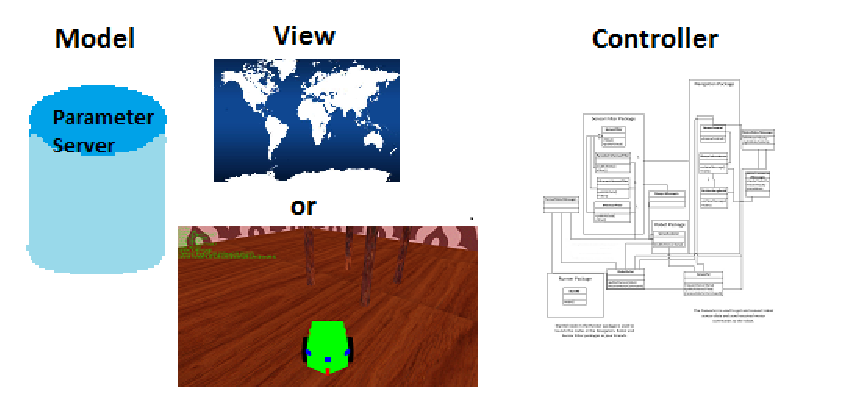
\includegraphics[scale=0.6]{images/MVC}
\par\end{centering}

\caption{\label{fig:MVC}The model of the system is stored in the parameter
server. The view can be either the world or the simulator. The controller
portion is described by the classes in the design model. }

\end{figure}


Figure \ref{fig:Simplified-Design-and} illustrate how the classes
in the design communicate using ROS messages. The communication begins
with the Converter or RobotActor class obtaining sensor readings and
ending with the robot's motors moving.

%
\begin{figure}[H]
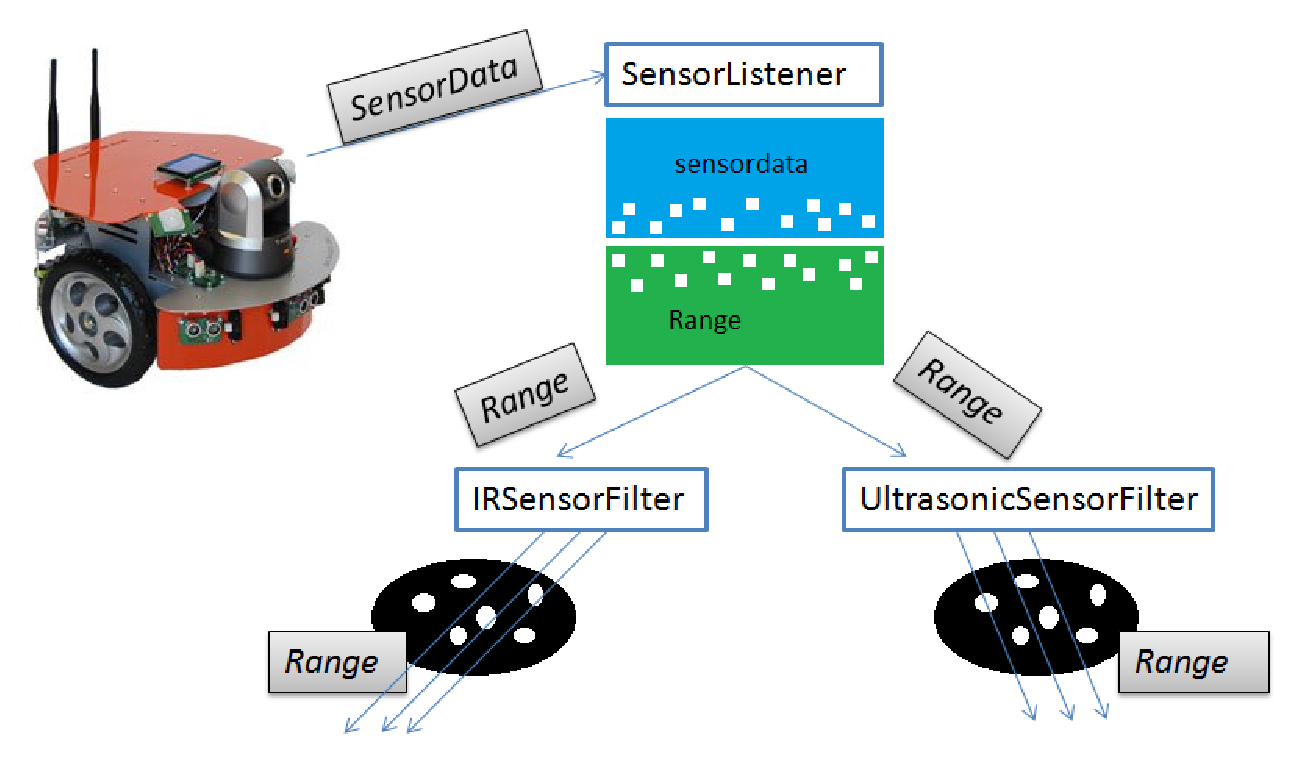
\includegraphics[scale=0.35]{images/SensorComm}\includegraphics[scale=0.45]{images/obstAvoid\lyxdot PNG}

\caption{\label{fig:Simplified-Design-and}Simplified communication model between
classes.}

\end{figure}


The design is centered around the Converter and the RobotActor classes
seen in figure \ref{fig:MainClasses}. Converter and RobotActor are
interchangeable bridges between the view and the control. Converter
is used when the robot is running in the real world and RobotActor
is used when using the simulator. They both publish SensorData messages
as seen in the first image in figure \ref{fig:Simplified-Design-and}.
SensorData messages include the range values of each of the robot's
sensors. Also, both classes respond to the MotorData message by sending
a command to actuate the robot\textquoteright{}s motors seen in the
second image of figure \ref{fig:Simplified-Design-and}. The MotorData
message contains the required left and right motor velocity. The SensorListener
class subscribes to the SensorData messages being published by a bridge
class, such as RobotActor, and publishes converted SensorData messages
in the ROS standard Range message type.

%
\begin{figure}[H]
\begin{centering}
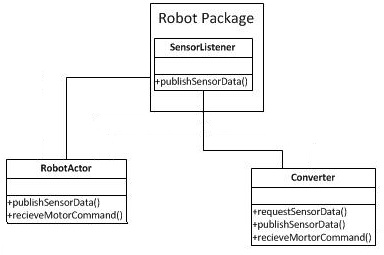
\includegraphics[scale=0.65]{images/mainClasses}
\par\end{centering}

\caption{\label{fig:MainClasses}SensorListener class uses SensorData messages
from either RobotActor or Converter.}



\end{figure}


SensorFilter is an abstract class that defines the methods for functionality
that any sensor filter should have. Therefore, for each of the sensor
types on the robot a filtering class is defined as seen in figure
\ref{fig:SensorFilter}. 

%
\begin{figure}[H]
\begin{centering}
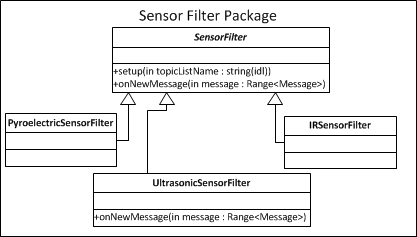
\includegraphics[scale=0.8]{images/SensorFilterPackage}
\par\end{centering}

\caption{\label{fig:SensorFilter}Diagram of the Sensor Filter package.}



\end{figure}


As shown in figure \ref{fig:Simplified-Design-and} the IRSensorFilter
and UltrasonicSensorFilter classes publish a filtered Range message.
Next, the ultrasonic and infrared instances of the BraitenburgAvoid
class subscribe to the corresponding filtered Range messages. The
filtered Range data is used to publish a MotorCommand message to avoid
obstacles based on the Braitenburg aggression behavior algorithm.
The MotorCommand message describes the linear and angular velocity
of the robot, as well as contains a priority field. The ObstacleAviodance
class subscribes to the MotorCommand messages sent by the infrared
and ultrasonic instances of the BraitenburgAvoid class. ObstacleAvoidance
class uses those MotorCommand messages and combines them into a single
MotorCommand. Finally, the MotorControl class subscribes to MotorCommand
messages published by ObstacleAvoidance and converts them into a MotorData
message. MotorControl also acts as an arbiter by only publishing the
highest priority MotorData message and as a gateway back to the Converter
or RobotActor classes.

%
\begin{figure}[H]
\begin{centering}
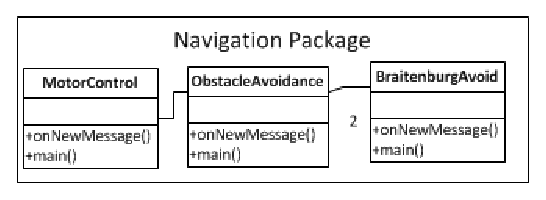
\includegraphics[scale=0.8]{images/NavigationPackage}
\par\end{centering}

\caption{\label{fig:NavigationPackage}Diagram of the Navigation package.}

\end{figure}



\subsection*{Simulator Design}

The initial design of the simulator relied on existing code which
supported only one Player with one graphical view; this code was later
adapted to support an arbitrary number of Actors, each with any number
of Sensors as seen in figure \ref{fig:SimDiagFig}. Each of the ultrasonic
and infrared sensors as well as the graphical displays were added
into the new system as individual instances of the Sensors attached
to the Actor. Multiple actors allow the user to view the environment
from the perspective of the robot or from an independent Camera actor;
they also allow Obstacle actors to be positioned in real-time. 

%
\begin{figure}[H]
\begin{centering}
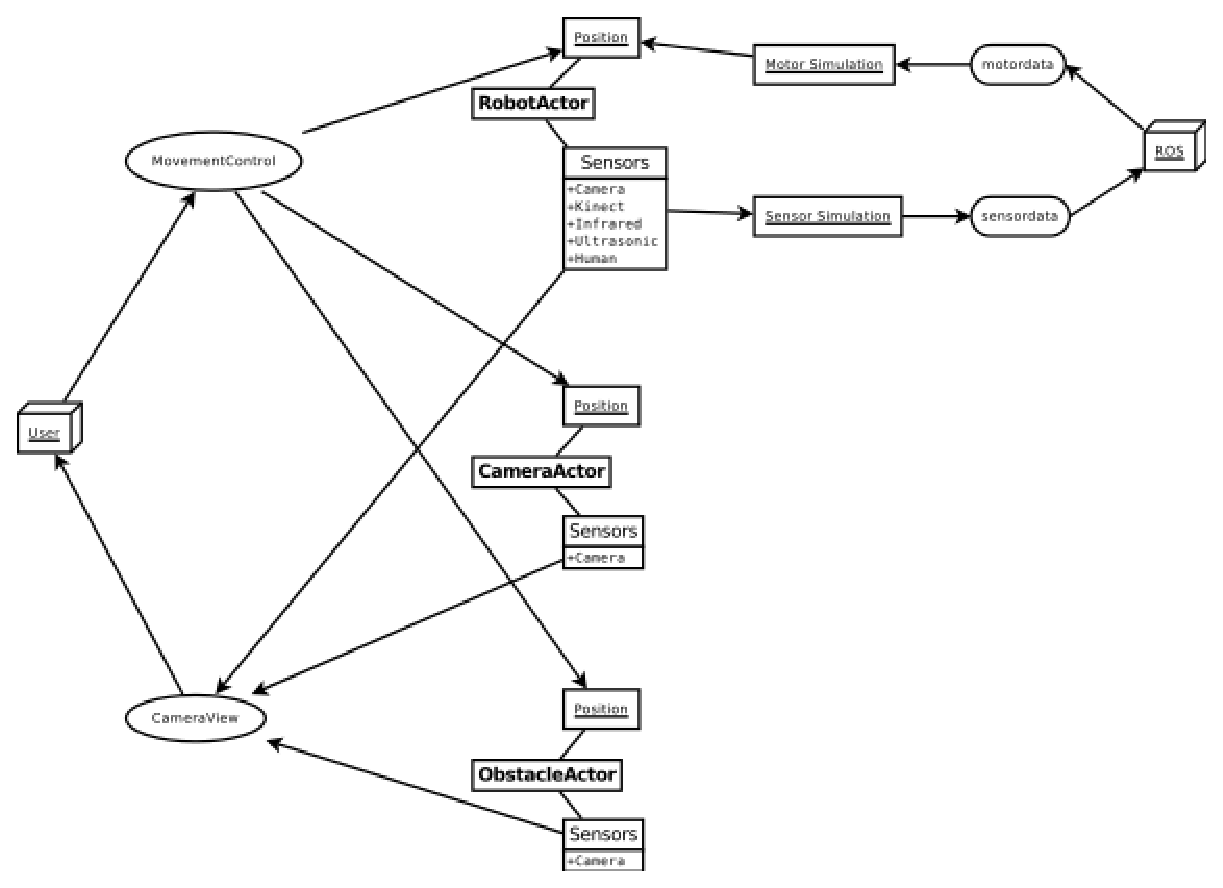
\includegraphics[scale=0.5]{images/Sim}
\par\end{centering}

\caption{\label{fig:SimDiagFig}The User can select to control any Actor's
position. The specific sensor the CameraView is rendered from can
also be selected. Data from ROS is also used to control the RobotActor's
position and the Sensors are output back to ROS.}

\end{figure}



\part*{Implementation}

The implementation of the design was completed in both C++ and Java.
C++ was used for the simulator, gesture recognition, and the serial
communication between the robot and Beagleboard. Java was used to
implement the rest of the design which includes a converter to standard
ROS message data-types, an ultrasonic sensor filter, obstacle avoidance
algorithm, and motor control arbiter.

The serial library used the PMS5005 protocol which allows any processor,
DSP, or PC to control the robot through the Universal Asynchronous
Receiver/Transmitter (UART) communication interface. The basic packet
outline, shown in Figure \ref{fig:Packet-format-for}, handles both
the sensor and motor data transmission. The library that implements
this interacts with ROS by subscribing to motor controls and publishing
sensor data. Using this packet structure, a large amount of information
can be processed every tick.

%
\begin{figure}[H]
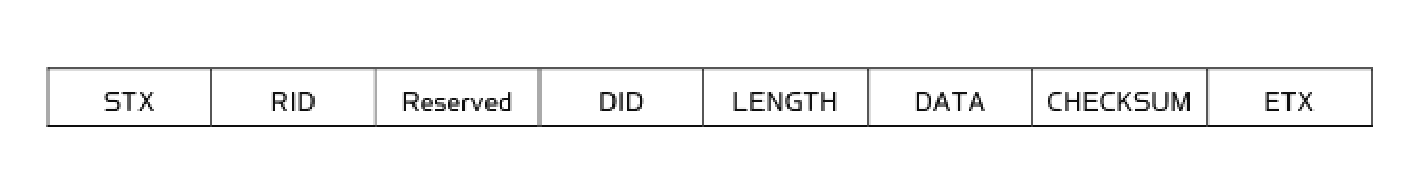
\includegraphics[scale=0.5]{images/packet}

\caption{\label{fig:Packet-format-for}Packet format for serial library}

\end{figure}


The sensor and motor data from the packet structure were not ideal
for our purposes and needed to be converted to useful formats. The
data for the sensors needed to be handled differently for each type
of sensor. The ultrasonic sensors were the most straightforward since
the control board returned the distance in the range of 0 - 255 cm,
which is already in the correct units for the message. The infrared
sensors needed to be converted since they return a non-linear voltage
value corresponding to a range of 10 - 80 cm. The voltage output
with respect to distance is shown in Figure \ref{fig:Infrared-sensor-voltage}.
This voltage output needed to be linearized using an interpolation
equation \cite{:LinearizingSharpRangerData}. The result of such an
equation with respect to Analog/Digital Converter (ADC) values is
shown in Figure \ref{fig:Linear-interpolation-of}. After testing
the human sensors, it was decided that these will not be used at this
point due to unreliable results.

%
\begin{figure}[H]
%
\begin{minipage}[t]{0.45\columnwidth}%
\begin{center}
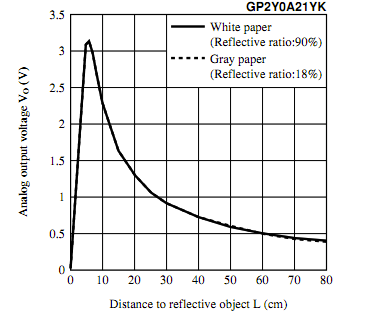
\includegraphics[scale=0.55]{images/voltageOutput}
\par\end{center}

\caption{\label{fig:Infrared-sensor-voltage}Infrared sensor voltage output
from \cite{:SharpGPYAY} values from \cite{:LinearizingSharpRangerData}}
%
\end{minipage}\hfill{}%
\begin{minipage}[t]{0.45\columnwidth}%
\begin{center}
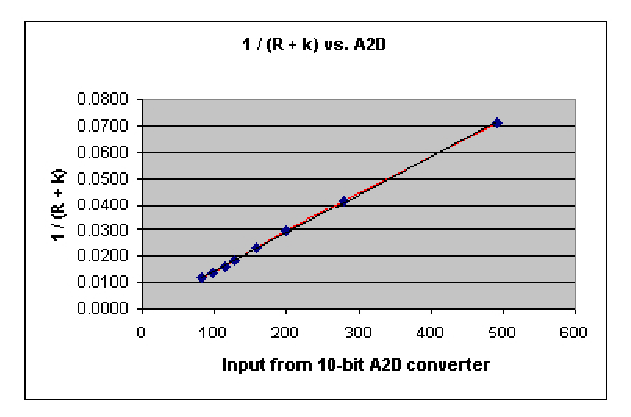
\includegraphics[scale=0.65]{images/ADCValues}
\par\end{center}

\caption{\label{fig:Linear-interpolation-of}Linear interpolation of Voltage
with respect to ADC}
%
\end{minipage}
\end{figure}


Once the serial library and sensor conversions were implemented on
a desktop system, the next step was to achieve this functionality
on the Beagleboard. The Beagleboard was loaded with Ubuntu 11.10 since
this OS works best with ROS. Some of the configuration scripts for
ROS require Internet access so a wireless internet connection was
part of the Beagleboard setup. ROS was compiled from source on the
Beagleboard because cross compiling is not recommended for ROS yet.
After configuring the installation, it quickly became apparent that
the overhead associated with ROS was more than expected. At the moment,
the Beagleboard is unable to support ROS at 10 Hz and further testing
will conclude whether this can be fixed or not.


\subsection*{High Level Software}

The Braitenburg obstacle avoidance algorithm produces linear and angular
velocity values, but the robot requires left and right wheel velocities
which can be converted using the differential drive kinematics equations
\ref{eq:LeftVelocity} and \ref{eq:RightVelocity}. Note that $\alpha_{S}(t_{k})$
and $\beta_{S}(t_{k})$ are normalized linear and angular velocities
defined in equations \ref{eq:translationalSpeed} and \ref{eq:rotationalSpeed}
and d is the wheel base of the robot.

\begin{equation}
V_{L}=\frac{2\alpha_{S}(t_{k})+d\beta_{S}(t_{k})}{2}\label{eq:LeftVelocity}\end{equation}


\begin{equation}
V_{R}=V_{L}-d\beta_{S}(t_{k})\label{eq:RightVelocity}\end{equation}


Ultrasonic sensors were used to provide obstacle avoidance, however
the sensors can overestimate the distance to a flat wall due to specular
reflection as seen in figure \ref{fig:Specular-reflection-of}. Over
estimation can happen when the sonar bounces off the wall and never
returns back to the sensor causing the robot to believe that there
is free space in front of it. 

%
\begin{figure}[H]
\begin{centering}
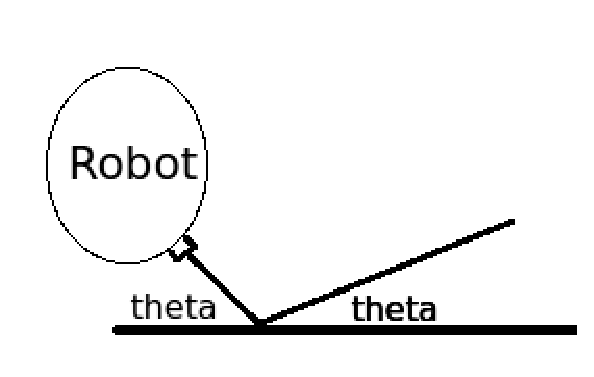
\includegraphics[scale=0.55]{images/sensorReflection}
\par\end{centering}

\caption{\label{fig:Specular-reflection-of}Specular reflection of ultrasonic
sensor.}

\end{figure}


These readings can be improved by applying an incremental filter (Equation
\ref{eq:USFilter}) as described in \cite{ran2005obsavothrbraaggbehmotfus}.
The filter works by acting as a short term memory to ensure that a
current reading of free space is correct based on the previous range.
For example, consider a robot that is approaching a wall as in figure
\ref{fig:Specular-reflection-of} and the readings are all less than
the max range of the sensor. Then specular reflection occurs causing
a max range reading. The filter in equation \ref{eq:USFilter} will
recognize the false max reading and use the previous filtered range
value instead.

\begin{equation}
\tilde{r_{i}}(t_{k})=\begin{cases}
r_{i}^{s}(t_{k}) & \textrm{if }r_{i}^{s}(t_{k})<r_{nr}^{s}\\
Min\{\tilde{r_{i}}(t_{k-1})+r_{\triangle},r_{nr}^{s}\} & \textrm{if }r_{i}^{s}(t_{k})=r_{nr}^{s}\end{cases}\label{eq:USFilter}\end{equation}


$r_{nr}^{s}$is the max range of the sensor, $r_{i}^{s}(t_{k})$ is
the current range measurement, $\tilde{r_{i}}(t_{k})$ is the current
filtered range value and $\tilde{r_{i}}(t_{k-1})$ is the previous
filtered value. $r_{\triangle}$ is a constant which is used to offset
the previous value and was chosen to be 20cm as described in \cite{ran2005obsavothrbraaggbehmotfus}. 

For every ROS node a new process is created, since a node is an executable.
Therefore, in the initial implementation of the project, every rosjava
node started a new process. However, the creation of new rosjava nodes
poses a problem due to the overhead of creating a new Java Virtual
Machine (JVM) for each node. A later implementation of rosjava implemented
the solution to the problem, which was to use a thread for each node,
rather than creating a new process. By using threads to encapsulate
nodes, only one JVM was started. Therefore, decreasing both the launch
time and overhead of starting the nodes.

RGBDSLAM was selected as the main algorithm to implement mapping.
In order to take advantage of RGBDSLAM, the entire project had to
be downgraded from using ROS Electric to ROS Diamondback and from
using Ubuntu 11.04 to Ubuntu 10.10. RGBDSLAM allows a point cloud
of the environment to be created from the Kinect data as seen in Figure
\ref{fig:RGBD-point-cloud}. Once a point cloud was generated, it
could be converted to an OctoMap as seen in Figure \ref{fig:Octomap},
a 3D occupancy grid map that is developed from an octree. The OctoMap
is then sent to the 3D navigation algorithm so that the robot can
utilize the map.

%
\begin{figure}[H]
%
\begin{minipage}[t]{0.45\columnwidth}%
\begin{center}
\includegraphics[scale=0.3]{\string"images/rgbdslam point cloud fig 1\string".eps}
\par\end{center}

\caption{\label{fig:RGBD-point-cloud}RGBD point cloud}
%
\end{minipage}\hfill{}%
\begin{minipage}[t]{0.45\columnwidth}%
\includegraphics[scale=0.3]{\string"images/octomap fig 2\string".eps}

\caption{\label{fig:Octomap}Octomap}
%
\end{minipage}
\end{figure}


The original goal was to have the robot using a static OctoMap to
navigate his environment, and eventually implement dynamic mapping
so the robot would have been able to map his environment while he
wandered. Due to issues with ROS running in a timely matter on the
Beagleboard, it is unsure as to whether the OctoMaps will be usable.
At this point, a sign language feature may be replacing the OctoMaps,
but that will be more-so determined in the final paper.

One of the initial challenges encountered in writing the simulator
was that the position of the robot was represented as a point on an
X-Y plane, but the input coming in from ROS would be in the form of
differential wheel movement commands. Finding the necessary equations
proved to be a challenge. It was also difficult to test initially
since the ROS interface had not yet been implemented to a working
degree. Some revisions and corrections had to be done once it was
possible to send specific commands from ROS and to observe whether
the resultant location of the robot in the simulation was correct.

%
\begin{figure}[H]
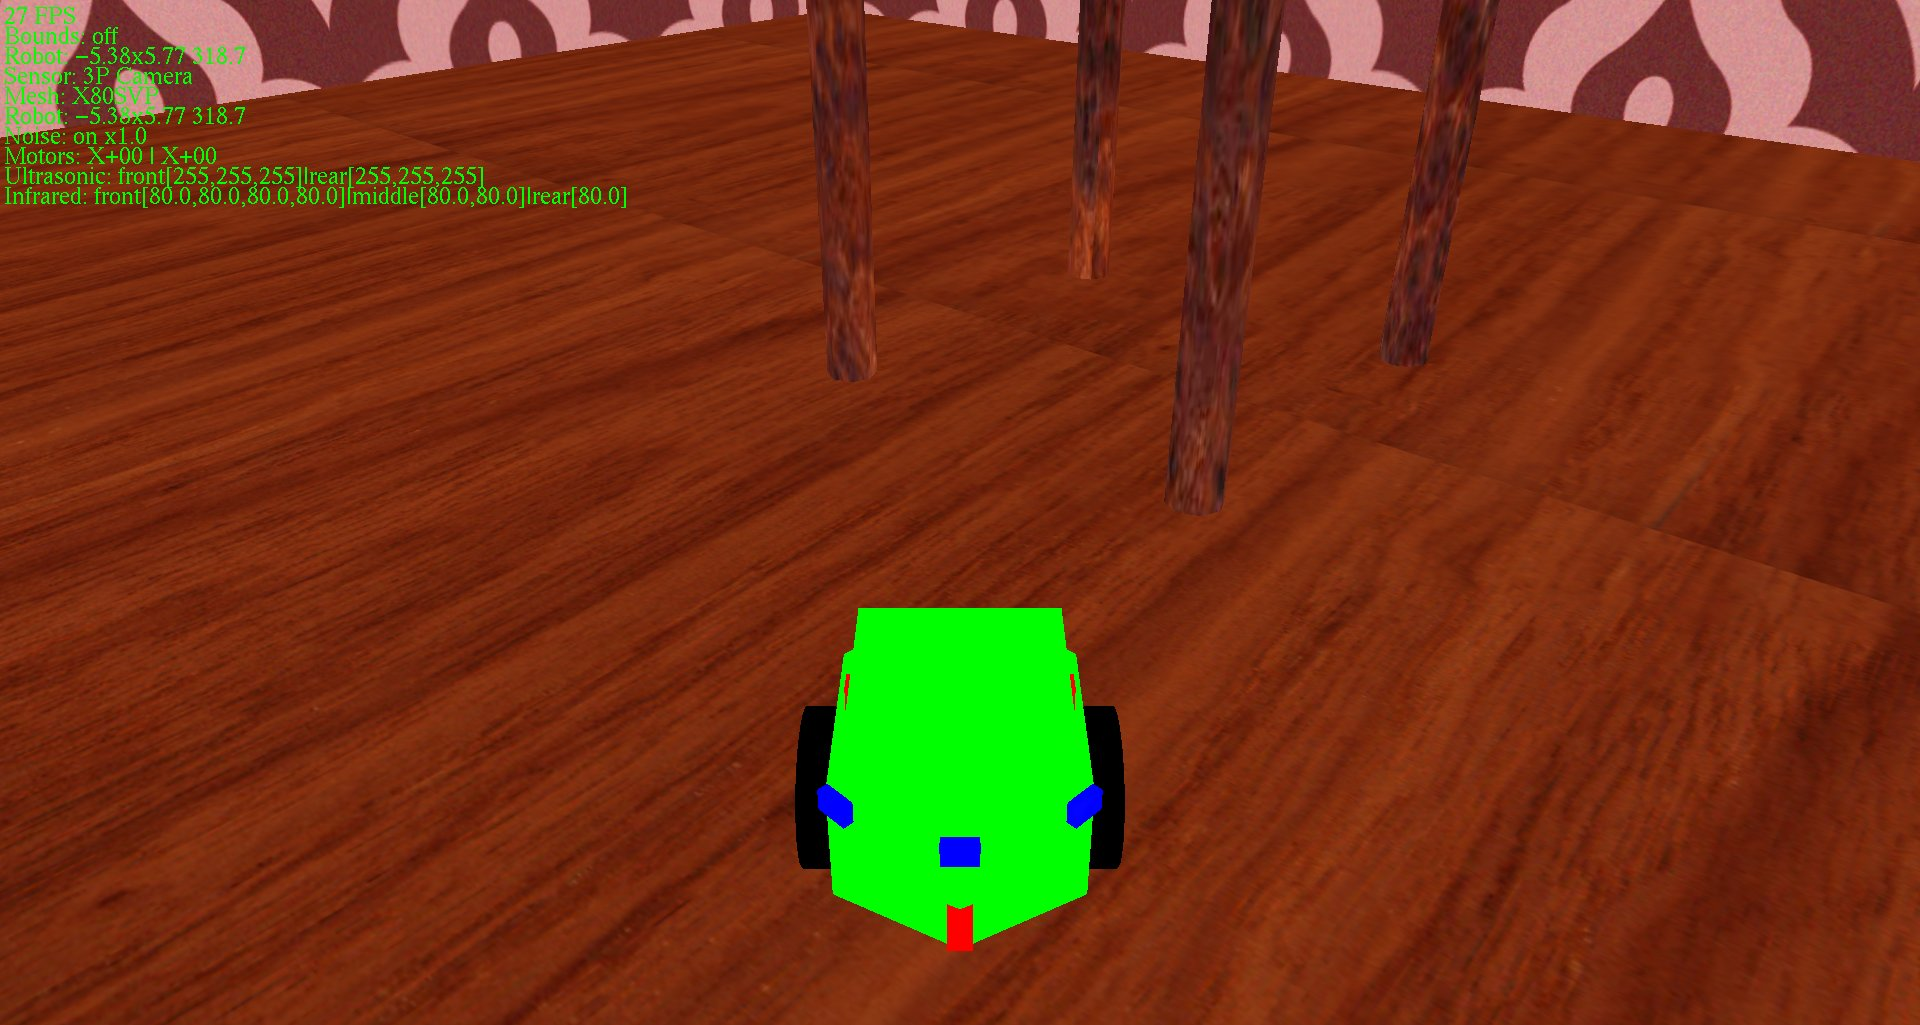
\includegraphics[scale=0.2]{images/3rdperson}

\caption{Simulator in third person view}

\end{figure}


There were also additional problems to address with respect to speed
and optimizing conversions of depthmap and point cloud data. One of
these problems was in computing a linear representation of the depth
map because GL uses a logarithmic representation when rendering, while
the Kinect provides a linear one. The initial implementation was very
inefficient in that it did the per-pixel transformations once for
each needed source, including the visual display, and ROS topics for
depth maps in two formats and the point cloud. This was improved significantly
by making the simulator render the scene once, at the Kinect hardware's
resolution. The conversion was done to this and scaled to fit the
size of the visualization window rather than doing the render and
conversion another time. There was also a large performance penalty
to doing the conversions for each output in separate loops. This required
a major refactor of the code to merge all of the conversion loops.
The final version was further optimized by tracking what ROS topics
are in use and only computing the data necessary to publish them.

%
\begin{figure}[H]
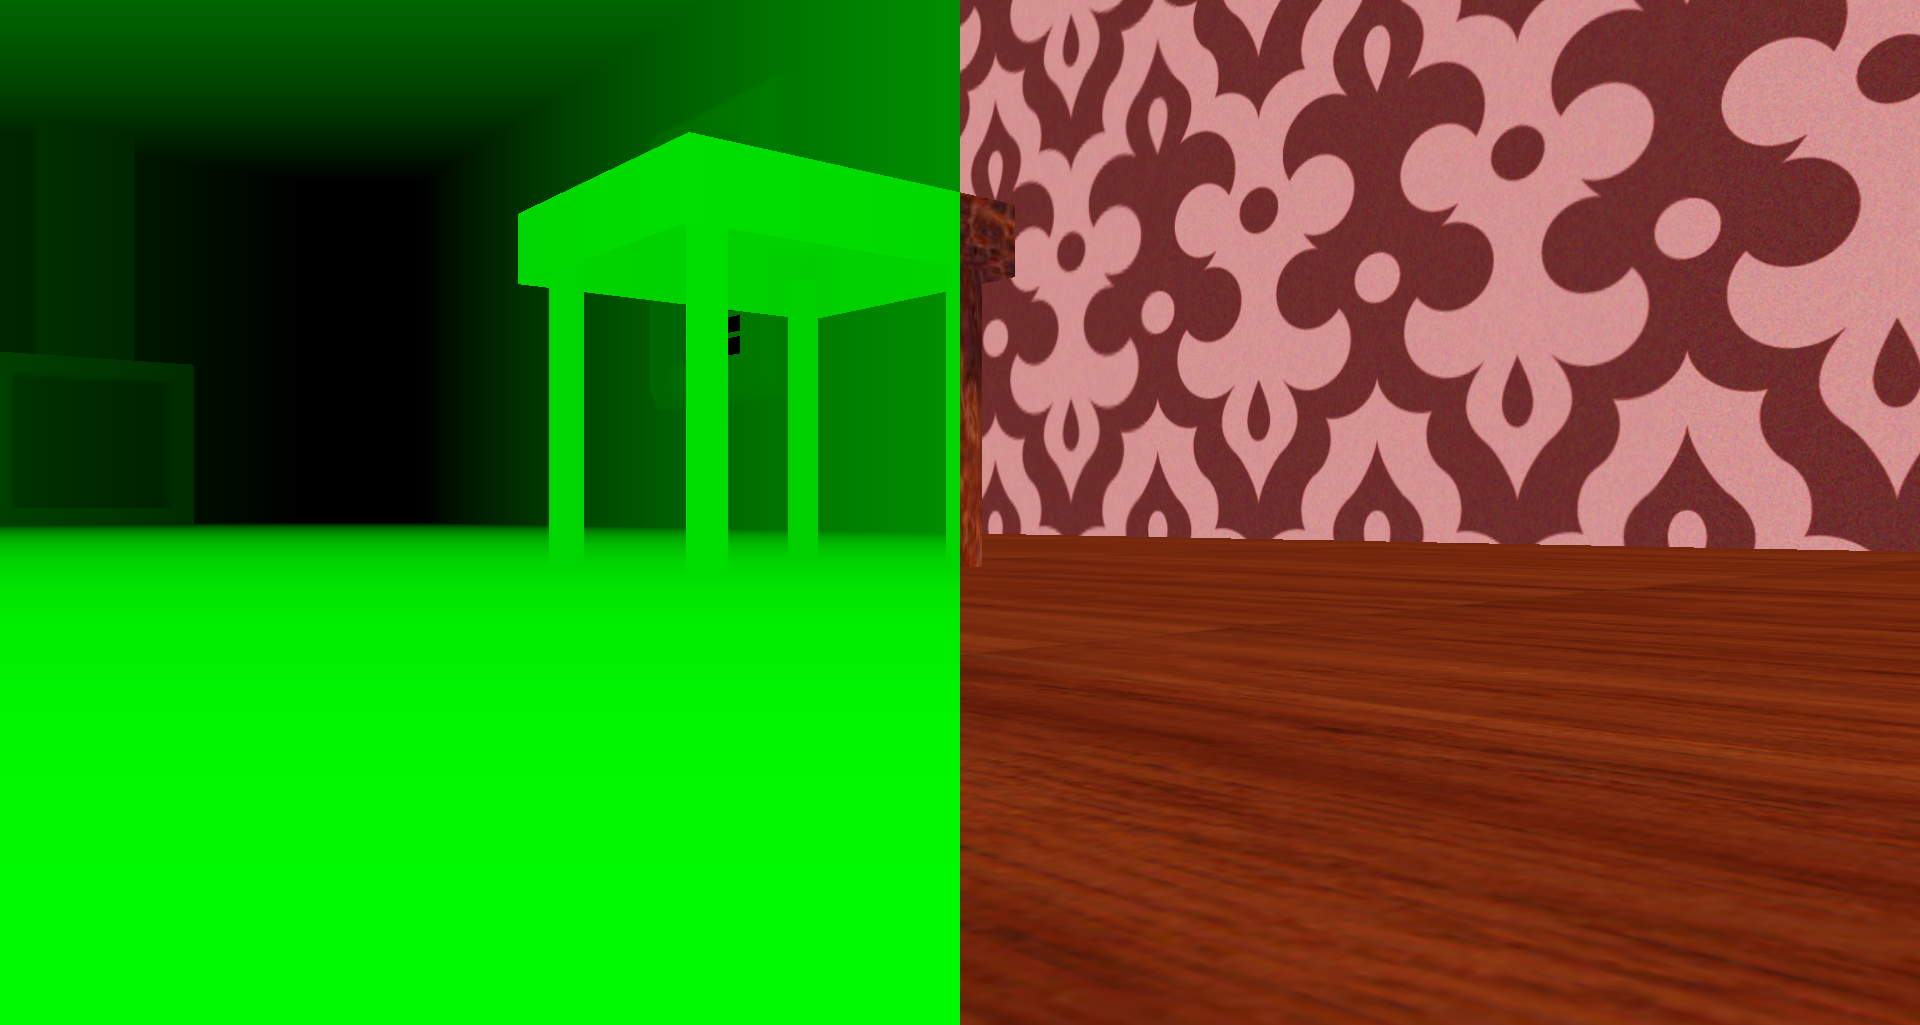
\includegraphics[scale=0.2]{images/depthmap}

\caption{Simulated Kinect depth map}

\end{figure}


There were also some modifications in what is rendered during each
pass. The simulator visualization targets a frame rate of 30 fps,
which is necessary for the visual output and Kinect video data simulation,
but was unable to attain that rate on the workstation with all rendering
passes active. Since the Sensing/Motion Controller on the robot only
functions at 10 Hz, it is only necessary to broadcast sensor data
to ROS at that rate; thus, the rendering passes needed for computing
sensor data could be skipped on 2/3rds of the frames, saving processing
resources and boosting frame rate. A useful optimization here would
be the ability to do the rendering passes asynchronously, which would
allow for less jitter in the frame rate caused by the combined passes
doing unequal amounts of work, however this would require a machine
with dual graphics cards.


\part*{Future Work}

In the future, there are plans to implement features such as more
advanced gesture recognition, a multi-agent system of physical robots,
and using rosjava on Android to teleoperate the robot.

Gesture recognition is one of the more immediate future plans for
the robot. A ROS stack called hand\_interaction, created by the Massachusetts
Institute of Technology, appears to be the best option for implementing
this feature. Using hand\_interaction, the location of the hands can
be determined. As a gesture is made, the movement of the hands will
be tracked and used to control the robot's behavior.

The system could be extended by adding robots, such as TurtleBots,
to create a multi-agent system. Capture the flag could be a way to
explore algorithms involved in multi-agent systems. However, due to
the limited processing power of the Beagleboard, there would be considerable
challenges implementing efficient navigation, SLAM, and learning algorithms.
One solution would be to use a remote computer to perform these features.

Another way the system could be extended is by using the Kinect for
facial and object recognition. This would allow for high level behavior
and learning rather than the current reactive-based system; however,
the processing capabilities of an on-board computer may be overwhelmed.

A future system could also utilize rosjava\textquoteright{}s ability
to operate on Android to provide a user with the ability to teleoperate
the robot or provide the robot access to the cloud.

\pagebreak{}

\bibliographystyle{plain}
\nocite{*}
\bibliography{bibliography}

\end{document}
